\section{Teste t de Student}
\begin{frame}{Teste t (de Student)}
 \begin{itemize}
   \item Teste não-viesado;
   \item O teste t (unilateral e bilateral);
   \item Teste t pareado;
   \item Teste t para duas amostras;
   \begin{itemize}
    \item Variâncias iguais (homogeneidade);
    \item Variâncias proporcionais.
   \end{itemize}
   \item Propriedades e exemplos;
   \end{itemize}
\end{frame}

\begin{frame}{Teste não-viesado}
 Em analogia com o conceito de estimador não-viesado, podemos também classificar testes de hipótese em viesados ou não-viesados.
 \begin{defn}[Teste não viesado]
 \label{def:unbiased_tests}
  Suponha que desejamos testar a hipótese
  \begin{align*}
   H_0 &: \theta \in \Omega_0, \\
   H_1&:  \theta \in \Omega_1. 
  \end{align*}
  através do teste $\delta$.
  Dizemos que $\delta$ é~\textbf{não-viesado} se (e somente se) para $\theta \in \Omega_0$ e $\theta^\prime \in \Omega_1$, vale 
  \[ \pi(\theta \mid \delta) \leq   \pi(\theta^\prime \mid \delta),\]
  ou seja, se a~\textit{função poder} é pelo menos tão grande no espaço onde $H_0$ é falsa ($\Omega_1$) quanto no espaço em que $H_0$ é verdadeira ($\Omega_0$). 
 \end{defn}
\end{frame}

\begin{frame}{Teste t: motivação}
 Suponha que estamos interessados em testar hipóteses sobre a média ($\mu$) de uma distribuição Normal quando a variância ($\sigma^2$) é desconhecida.
 Sabemos que é possível encontrar uma quantidade pivotal $(\Sm-\mu)/\hat{\sigma}^\prime$ tal que é possível construir um intervalo de confiança para $\mu$ da forma $\Sm - c\hat{\sigma}^\prime/\sqrt{n}, \Sm + c\hat{\sigma}^\prime/\sqrt{n}$, onde $c = T^{-1}(\gamma; n-1)$ é a f.d.a. inversa de uma distribuição t de Student com $n-1$ graus de liberdade.
 
 \begin{pergunta}[Como falar sobre $\mu$ quando ambas $\mu$ e $\sigma^2$ são desconhecidas?]
 \label{qst:unknown_mean_and_variance}
  Suponha que Palmirinha esteja interessada em testar a hipótese de que a média da concentração de amido na sua pamonha seja maior que $\mu_0 = 7 mg/L$, ou seja,
    \begin{align*}
   H_0 &: \mu \geq \mu_0, \\
   H_1&:  \mu < \mu_0,
  \end{align*}
  mas ela desconhece a variância do processo, $\sigma^2$.
  Como testar hipóteses sobre $\theta = (\mu, \sigma^2)$?
 \end{pergunta} 
\end{frame}

\begin{frame}{Exemplo}
 Palmirinha pode começar computando a estatística 
 \begin{equation*}
  U:= \sqrt{n}\frac{\Sm-\mu_0}{\hat{\sigma}^\prime},
 \end{equation*}
onde $\hat{\sigma}^\prime = \sqrt{\sum_{i=1}^n (X_i - \Sm)^2/(n-1)}$ como já estudado.
A partir daí, pode construir um teste $\delta_c$ que rejeita $H_0$ se $U \leq c$, para uma constante real $c$ definida.
\begin{obs}[A distribuição de $U$ sob $H_0$]
 Quando $H_0$ é verdadeira, em particular, quando $\mu = \mu_0$, $U$ tem distribuição t de Student com $n-1$ graus de liberdade, não importando o valor de $\sigma^2$.
 Isto é, $U$ é pivotal.
\end{obs}
\end{frame}


\begin{frame}{Caracterizando o teste t}
\begin{defn}[Teste t]
\label{def:Student_t_test}
Um teste $\delta_c$ que rejeita $H_0$ se $U\geq c$ (equiv. $U \leq c$), com $c = T^{-1}(1-\alpha_0; n-1)$ é chamado um teste t (unicaudal) de tamanho $\alpha_0$.
\end{defn}
\begin{theo}[Propriedades do teste t]
Suponha que $\delta_c$ rejeita $H_0$ se $U\geq c$.
Então
\begin{itemize}
 \item [i)] $\mu = \mu_0 \implies \pi(\mu, \sigma^2 \mid \delta_c) = \alpha_0$;
 \item [ii)] $\mu < \mu_0 \implies \pi(\mu, \sigma^2 \mid \delta_c) < \alpha_0$;
 \item [iii)] $\mu > \mu_0 \implies \pi(\mu, \sigma^2 \mid \delta_c) > \alpha_0$;
 \item [iv)] $\lim_{\mu \to -\infty}  \pi(\mu, \sigma^2 \mid \delta_c) = 0$;
 \item [v)] $\lim_{\mu \to \infty}  \pi(\mu, \sigma^2 \mid \delta_c) = 1$;
 \item [vi)] $\delta_c$ é não-viesado e tem tamanho $\alpha_0$.
\end{itemize}
\end{theo}
\textbf{Prova:} Ver Teorema 9.5.1. de DeGroot. 
\end{frame}

\begin{frame}{P-valor para o teste t}
 Lembre-se de que o p-valor é a probabilidade,~\textbf{sob $H_0$}, de observarmos uma estatística tão ou mais extrema do que a que foi observada.
 \begin{theo}[P-valor para um teste t unicaudal]
 \label{thm:pvalue_one_tailed}
 Suponha que observarmos $U = u$ e seja $T(\cdot; n-1)$ a f.d.a. de uma distribuição t de Student com $n-1$ graus de liberdade.
 Para a hipótese
\begin{align*}
   H_0 &: \mu \geq \mu_0, \\
   H_1&:  \mu < \mu_0,
  \end{align*}
o p-valor vale $T(u;n-1)$, enquanto para a hipótese
\begin{align*}
   H_0 &: \mu \leq \mu_0, \\
   H_1&:  \mu > \mu_0,
  \end{align*}
o p-valor vale $1-T(u; n-1)$.   
 \end{theo}
 \textbf{Prova:} Notar que $\delta_c$ depende de $c = T^{-1}(1-\alpha_0; n-1)$.
Ver Teorema 9.5.2 em DeGroot. 
\end{frame}

\begin{frame}{Teste t pareado: motivação}
Suponha que estamos interessados em medir o efeito de uma droga sobre a pressão arterial sistólica de um grupo de pacientes.
Suponha que medimos as pressões arteriais de $n$ pacientes antes ($\bX$) e depois ($\boldsymbol{Y}$) de administrar a droga.
Vamos supor que $X_i \sim\operatorname{Normal}(\mu_{\text{antes}}, \sigma^2)$ e $Y_i \sim\operatorname{Normal}(\mu_{\text{depois}}, \sigma^2)$.
\begin{figure}
 \begin{center}
  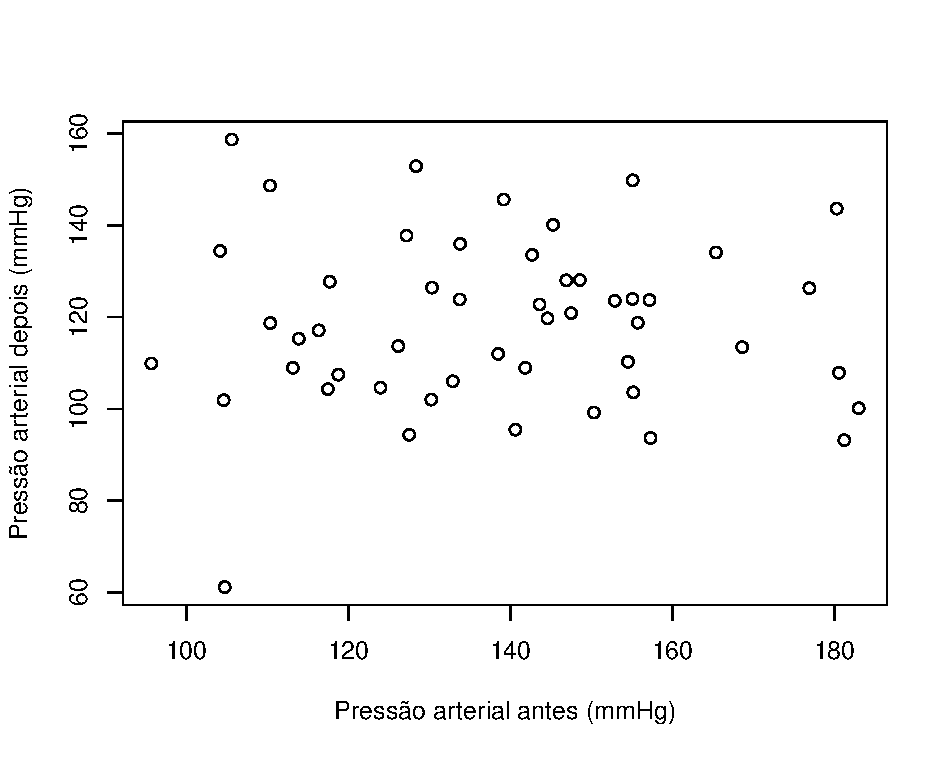
\includegraphics[scale=.5]{figures/blood_pressure.pdf}
 \end{center}
\end{figure}
\end{frame}

\begin{frame}{Teste t pareado: execução}
Estamos, portanto, interessados na hipótese\footnote{Note que, neste caso, esta é a hipótese razoável a ser testada, porque estamos interessados apenas em rejeitar a hipótese de que a droga~\textbf{não aumenta} a pressão arterial dos pacientes.
Drogas que não tem efeito ou causam aumento da pressão não costumam ser aprovadas pela ANVISA.}
\begin{align*}
   H_0 &: \mu_{\text{antes}} \leq \mu_{\text{depois}}, \\
   H_1 &:  \mu_{\text{antes}} > \mu_{\text{depois}}.
  \end{align*}

Podemos modelar a variável $Z_i = X_i-Y_i$ e sabemos que $Z_i \sim\operatorname{Normal}(\mu_Z = \mu_{\text{antes}}-\mu_{\text{depois}}, 2\sigma^2)$.
Desta forma, estamos interessados em testar hipóteses sobre $\mu_Z$ a partir de $\boldsymbol{Z}$.
Em particular, a hipótese acima se traduz em
\begin{align*}
   H_0 &: \mu_Z \leq 0, \\
   H_1 &: \mu_Z > 0,
\end{align*}
uma hipótese que podemos testar utilizando um teste t unicaudal como já discutido.
\end{frame}

\begin{frame}{Teste t para duas amostras}
Considere agora a situação em que dispomos de dois conjuntos de dados, $\boldsymbol{X} = \{X_1, X_2, \ldots, X_m\}$ e $\boldsymbol{Y} = \{Y_1, Y_2, \ldots, Y_n\}$ e queremos estudar diferenças nas médias.
Novamente, vamos modelar os processos como distribuições normais: $X_i \sim\operatorname{Normal}(\mu_1, \sigma_1^2), i = 1, 2, \ldots, m$ e $Y_j \sim\operatorname{Normal}(\mu_2, \sigma_2^2), j = 1, 2, \ldots, n$.

Sob a premissa de homogeneidade $\sigma_1^2 = \sigma_2^2 = \sigma^2$, podemos testar a hipótese
\begin{align*}
   H_0 &: \mu_1 \leq \mu_2, \\
   H_1 &: \mu_1 > \mu_2,
\end{align*}
computando a estatística 
\begin{equation*}
 U = \frac{\sqrt{m + n - 2}(\bar{X}_m - \bar{Y}_n)}{\sqrt{\left(\frac{1}{m} + \frac{1}{n}\right) (S_X^2 + S_Y^2)}},
\end{equation*}
onde $\bar{X}_m = (1/m)\sum_{i=1}^m X_i$,  $\bar{Y}_n = (1/n)\sum_{j=1}^n Y_j$, $S_X^2 = \sum_{i=1}^m (X_i-\bar{X}_m)^2$ e $S_Y^2 = \sum_{j=1}^n (Y_j-\bar{Y}_n)^2$.
\textbf{O teste procede analogamente ao que já foi discutido}.
\end{frame}

\begin{frame}{Relaxando a premissa de homogeneidade}
Até aqui assumimos variâncias iguais, tanto no teste pareado quanto no teste para duas amostras. 
Podemos relaxar a premissa de igualdade das variâncias um pouco se assumirmos que $\sigma_2^2 = k\sigma_1^2$, isto é, que a razão entre as variâncias é conhecida.
Neste caso, a estatística teste vale
\begin{equation*}
 U_k = \frac{\sqrt{m + n - 2}(\bar{X}_m - \bar{Y}_n)}{\sqrt{\left(\frac{1}{m} + \frac{k}{n}\right) (S_X^2 + \frac{S_Y^2}{k})}}.
\end{equation*}

Quando as variâncias são diferentes e desconhecidas e não conhecemos $k$, temos o problema de Behrens-Fisher\footnote{Em homenagem ao químico alemão Walter-Ulrich Behrens (1902--1962) e ao biólogo e estatístico britânico Ronald Aylmer Fisher (1890-1962).} que é muito mais difícil de tratar.
\end{frame}

\begin{frame}{O teste t bicaudal (bilateral)}
No caso do  teste t pareado, podemos estar interessados apenas em testar $\mu_{\text{antes}}= \mu_{\text{depois}}$, o que levaria a uma hipótese alternativa composta e um teste bicaudal (bilateral).
Situação parecida acontece no caso de duas amostras quando queremos testar $\mu_1 = \mu_2$.
Nesses casos, podemos facilmente adaptar os testes discutidos para acomodar a hipótese bilateral.
Em ambos os casos, podemos fazer o teste ``rejeite $H_0$ se $|U|\geq T^{-1}(1-\alpha_0/2; n-1)$'', e este terá tamanho $\alpha_0$.
\begin{figure}
 \begin{center}
  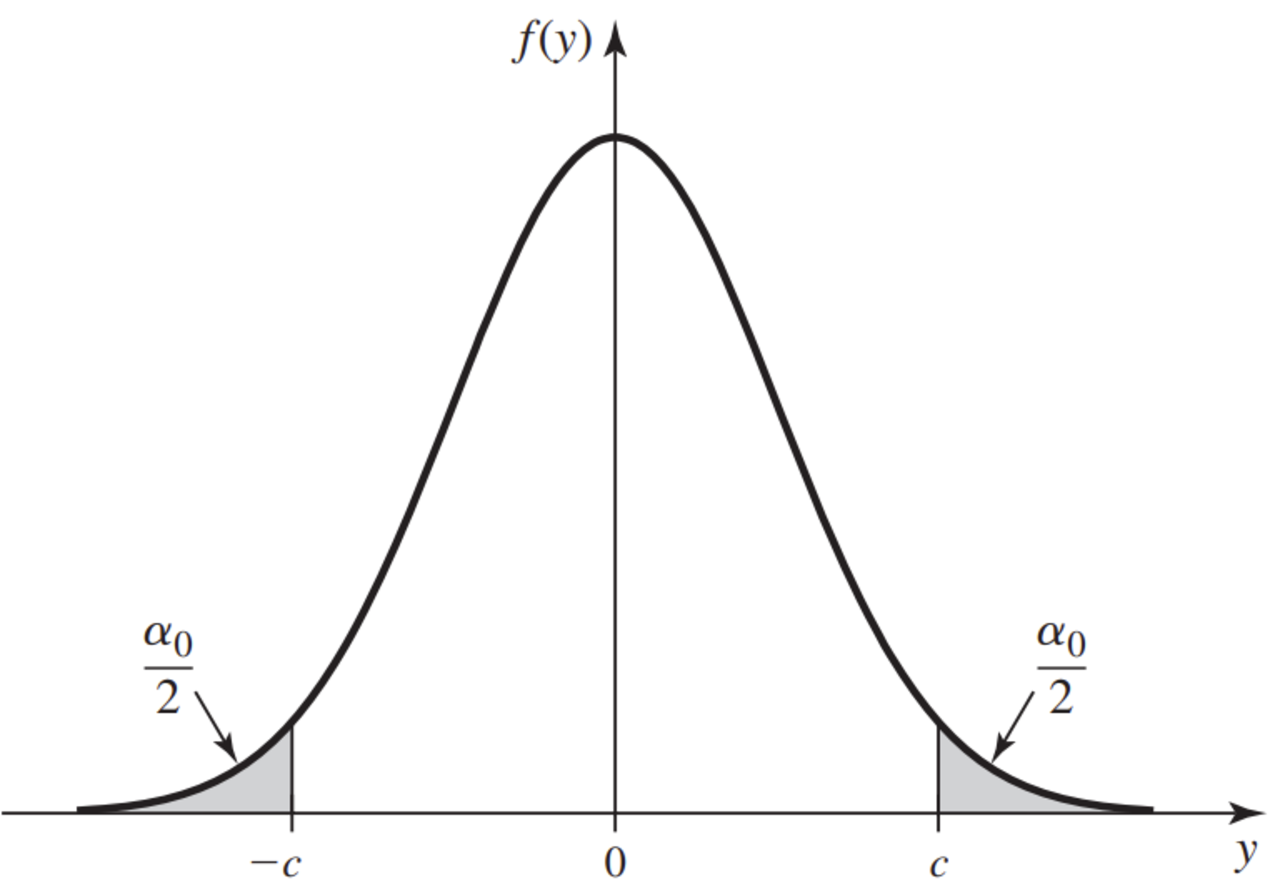
\includegraphics[scale=0.3]{figures/bilateral.pdf}
 \end{center}
\end{figure}
\end{frame}

\begin{frame}{O Teste t como um TRV (LRT)}
Podemos também entender o teste t como um teste de razão de verossimilhanças.
Em particular, temos para um teste t unicaudal, 
\begin{align*}
 \Lambda(\bx) &= \frac{\sup_{(\mu, \sigma^2):\mu \geq \mu_0} f_n(\bx \mid \mu, \sigma^2) }{\sup_{(\mu, \sigma^2)} f_n(\bx \mid \mu, \sigma^2)}, \\
 &=  \begin{cases}
     \left(\frac{\hat{\sigma^2}}{\hat{\sigma_0^2}}\right)^{n/2} \: \text{se} \: \sm> \mu_0,\\
     1,\:\text{caso contrário},
\end{cases} 
\end{align*}
onde $\hat{\sigma^2}$ é o EMV da variância e $\hat{\sigma_0^2} = \frac{1}{n}\sum_{i=1}^n (x_i-\mu_0)^2$.
Onde o teste t tradicional rejeita $H_0$ se $U\geq c$, sua formulação TRV rejeita $H_0$ se $\Lambda(\bx) \leq k$.
A relação entre $c$ e $k$ é 
\begin{equation*}
 c = \sqrt{\left[\left(\frac{1}{k^2}\right)^{1/n} - 1 \right](n-1)}, 
\end{equation*}
o que estabelece que o teste t é um teste de razão de verossimilhanças.
\end{frame}

\begin{frame}{O que aprendemos?}
\begin{itemize}
  \item[\faLightbulbO] O teste t permite comparar a média de um conjunto de dados com um valor postulado $\mu_0$;    
  \item[\faLightbulbO] Permite também comparar as médias de duas amostras, pareadas ou independentes;
  \item O teste t é não-viesado e pode ser escrito como um teste de razão de verossimilhanças;
   \end{itemize}
 \end{frame}

\begin{frame}{Leitura recomendada}
\begin{itemize}
 \item[\faBook] DeGroot seções 9.5 e 9.6;
 \item[\faBook] $^\ast$ Casella \& Berger (2002), seção 8.
 \item[\faForward] Próxima aula: DeGroot, seção 9.7;
 \item {\large\textbf{Exercícios recomendados}}
  \begin{itemize}
   \item[\faBookmark] DeGroot Seção 9.5: exercício 8.
  \end{itemize}
 \end{itemize} 
\end{frame}
